% ============================================================================
% 中文完整版（草稿）
% 与 paper/neurips2026/main.tex（英文投稿版）逐节对应，数字完全一致。
% 编译：tectonic -X compile main_zh.tex --outdir .  （自动获取 Fandol 中文字体）
% 图片复用英文版的 figures/（图内标签仍为英文；如需中文图内文字可另行本地化）。
% ============================================================================
\documentclass[UTF8,11pt]{ctexart}

\usepackage[a4paper,margin=2.4cm]{geometry}
\usepackage{graphicx}
\usepackage{booktabs}
\usepackage{tabularx}
\usepackage{subcaption}
\usepackage{amsmath}
\usepackage{amssymb}
\usepackage{url}
\usepackage[round]{natbib}
\usepackage[colorlinks=true,linkcolor=blue,citecolor=blue,urlcolor=blue]{hyperref}

% 放宽浮动体参数，避免 [H] 强制浮动在密集中文排版中留下大幅空白
\renewcommand{\topfraction}{0.95}
\renewcommand{\bottomfraction}{0.95}
\renewcommand{\textfraction}{0.05}
\renewcommand{\floatpagefraction}{0.9}
\setcounter{topnumber}{4}
\setcounter{bottomnumber}{4}
\setcounter{totalnumber}{8}

\graphicspath{{../neurips2026/figures/}}

% 百分点宏（与英文版一致）
\newcommand{\pp}{\ensuremath{\,\mathrm{pp}}}

\title{非线性知识图谱能否使小模型的长上下文阅读器逼近证据上限?\\
---基于侦探小说的案例研究}

\author{匿名作者 \\
匿名单位 \\
\texttt{anon@example.com}}

\begin{document}
\maketitle

\begin{abstract}
大语言模型将长文档当作\textbf{线性}输入历史来阅读：token 按叙述顺序进入固定
上下文窗口，因此证据的可及性既取决于相关性、也取决于位置。我们研究一个
\textbf{非线性}检索系统——文本之上的知识图谱``思维导图''——能否让小型上下文
模型逼近证据本身所允许的上限。我们在 30 部侦探小说、234 道多项选择题上，为每部
小说冻结一个离线知识图谱，并在固定 9B 本地模型、16\,K 上下文的条件下，将三种
图谱导航协议分别与尾窗口基线、整书压缩基线、向量检索(RAG)基线和仅题目对照进行
比较。30 部小说来自两条不同的冻结图谱构建流水线，因此合并数字仅具描述性。
去偏金标预言机——在去除选项位置伪影的协议下向模型展示全部官方线索段——达到
54.7\%，而仅题目对照为 40.2\%（配对 +14.53\,\pp{}，$p=0.0005$）。图谱引导的
证据扩展达到 53.8\%，与预言机在统计上不可区分（$p=0.912$），尽管每题只读取
若干图谱选出的段落。我们还表明，选项在前的预言机运行不是可靠上限：当金标答案为
D 时它正确率为 79.4\%，但对 A--C 只有 21.8--40.0\%，这是去偏协议能够消除的
选项位置锚定伪影。更广泛地说，我们把图谱导航视为\textbf{非线性结构化记忆}的一种
实例——一种模型可以跳跃穿行的稀疏索引，使推理依赖结构而非位置。我们预期这一原语
在上下文窗口增长到百万 token、而文档与长期记忆再大几个数量级时会更加重要。
\end{abstract}

\textbf{关键词：}长上下文推理；知识图谱检索；非线性结构化记忆；小型语言模型；
多项选择评估

% ============================================================================
\section{引言}
\label{sec:intro}

LLM 的上下文窗口是一段线性历史：模型逐 token 观察文档，在固定长度的窗口中
决定关注什么。对于一部约 50 万字符（约 $10^5$ token，远大于 16\,K 上下文）的小说，
``凶手为何留下罐头茶''的答案可能位于 0.28 附近的段落，而模型的有效注意力被钉在
尾部附近
\citep{liu2024lost,hsieh2024found}。因此检索问题不是``证据是否存在''，而是
``阅读器能否非线性地导航到它''。检索增强生成 \citep{lewis2020rag} 通过扁平的
相似度索引缓解了这一问题，但它仍把文档当作一段待切分的字节流。

本文研究另一种原语：\textbf{图谱导航}。小说之上的知识图谱——人物、地点、线索
物品、事件、时间锚点，以及提到它们的证据句，由带类型的边相连——是一张非线性
的``思维导图''。回答问题时不需在全文做线性扫描；模型可以从查询节点出发，跳到
一小簇证据节点，无论证据在线性文本中的位置如何，都能保持在很小的上下文预算内
（图~\ref{fig:schematic}）。本文的核心问题是：对于小型、本地、长上下文模型，
这种非线性图谱导航能否让模型逼近\textbf{金标上限}——即模型被交给全部官方线索段
时的准确率？该原语还能超越这一试验台：1M token 的上下文仍被 100M token 的语料或
长期记忆存储所压倒，那里的瓶颈正是我们这里研究的线性访问，而非窗口大小。

我们为此构建一个干净、冻结的基准。在 30 部侦探小说、234 道多项选择题上，我们
固定一个 9B 本地模型（16\,K 上下文、禁用思维链），并评估 (i)~基于冻结单书图谱
的三种图谱导航协议，(ii)~三种标准检索/压缩基线，(iii)~仅题目对照，以及
(iv)~\textbf{公平金标预言机}：在去除选项位置伪影的协议下向模型展示全部官方线索
段。我们测量图谱导航是否逼近预言机，并量化剩余差距的确切来源。

\begin{figure}[t!]
\centering
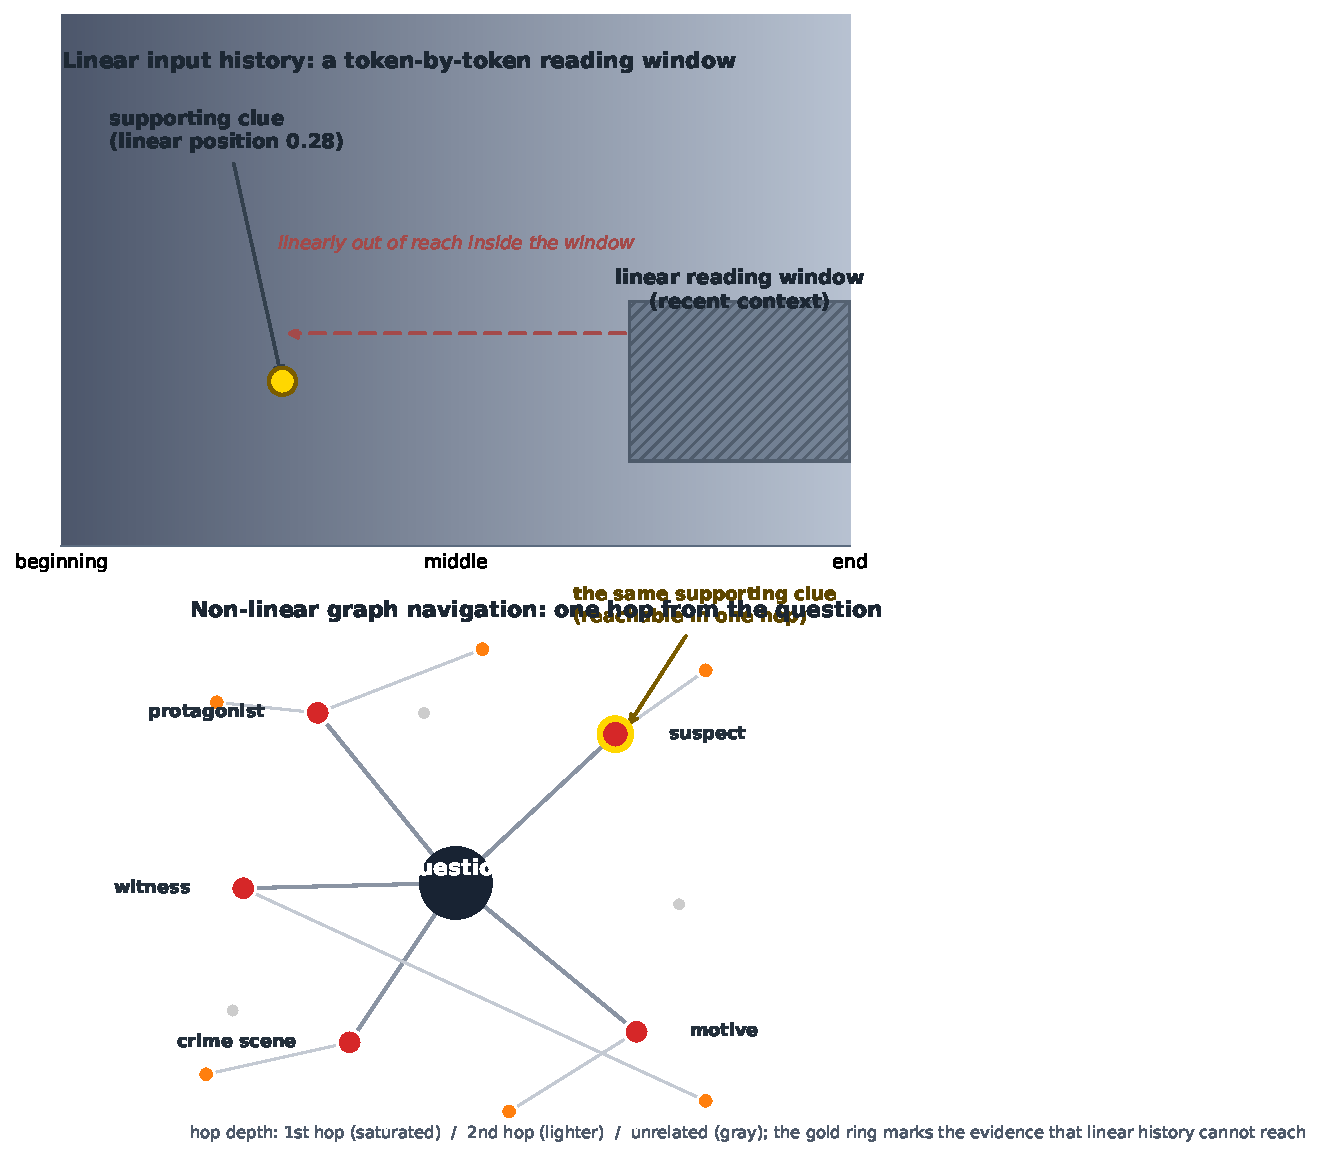
\includegraphics[width=0.8\linewidth]{fig_schematic_linear_vs_graph.pdf}
\caption{
线性输入历史 vs.\ 非线性图谱导航。\textbf{上：}小说是一条 $0$--$1$ 线性阅读尺；
尾部的固定大小阅读窗口看不到位于 0.28 处的支撑线索。\textbf{下：}同一条线索离
查询节点仅一步图跳，可用极小的上下文预算到达，与线性位置无关。跳数深度以大小和
颜色编码（一跳饱和、二跳更淡、无关节点为灰色），遵循我们分析中沿用的看板配色
约定。
}
\label{fig:schematic}
\end{figure}

我们的核心结果有三点。

\begin{itemize}
\item \textbf{去偏预言机是真正的上限。}在洗牌选项、证据在前的协议下，金标预言机
达到 54.7\%，而仅题目对照为 40.2\%（+14.53\,\pp{}，配对精确 McNemar
$p=0.0005$）；原始的选项在前金标运行只有 41.5\%，与仅题目对照（40.2\%）持平，
因为模型锚定于选项位置。
\item \textbf{图谱导航逼近上限。}图谱引导的证据扩展达到 53.8\%，与公平金标预言机
在统计上不可区分（$p=0.912$，在同一 234 题上配对），且仅使用图谱推导的证据。
三种图谱协议在更难的题目上都优于尾窗口基线。
\item \textbf{必须控制选项位置伪影。}公平金标预言机的 +14.5\,\pp{} 优势在选项在
前的预言机运行中完全不可见；把方法去比较一个未经去偏的预言机没有意义。
\end{itemize}

本文结构如下。第~\ref{sec:related}~节将该工作置于长上下文与图谱检索文献之中。
第~\ref{sec:method}~节描述三种图谱导航协议、基线与去偏金标协议。
第~\ref{sec:setup}~节详述冻结语料与统计方法。第~\ref{sec:results}~节报告主结果、
上限分析、选项位置伪影、队列异质性与难题表现。第~\ref{sec:discussion}~节讨论协议
不对称及其对小型模型图谱检索的意义，随后是局限（第~\ref{sec:limitations}~节）、
更广泛影响（第~\ref{sec:impact}~节）与结论（第~\ref{sec:conclusion}~节）。

% ============================================================================
\section{相关工作}
\label{sec:related}

\textbf{长上下文模型中的位置偏置。}LLM 在长输入上的表现随相关内容位置而退化：
模型偏好长上下文首尾的内容，在中部受损 \citep{liu2024lost}，跨模型家族也报告了
类似的中部塌陷与近因效应 \citep{hsieh2024found}。我们的尾窗口基线直接测量了
线索密集叙事中的近因先验；我们的去偏预言机则去除一个正交的伪影：多项选择评估中
的选项位置锚定。

\textbf{基于图谱的检索。}GraphRAG \citep{edge2024graphrag} 在实体图上构建社区
层次，并从聚合的社区摘要回答问题；HippoRAG \citep{gutierrez2024hipporag} 在知识
图谱上构建基于个性化 PageRank 的检索；GraphReader \citep{li2024graphreader} 用
一个智能体控制器在图上游走。这些系统面向大型前沿模型的开放问答，优化召回。
我们的设定有三点不同：图谱是冻结的离线工件（不按查询构建）；阅读器是固定 9B
本地模型、16\,K 上下文；结局是相对去偏证据上限的多项选择准确率，而非开放式生成。

\textbf{层次化与结构化记忆。}RAPTOR \citep{sarthi2024raptor} 为长上下文检索构建
递归摘要聚类的树；LongRAG \citep{zhao2024longrag} 检索长``组单元''把证据推入
上下文窗口。这些是文本的线性到树变换；我们的图谱额外编码带类型的关系与实体解析，
并且我们把检索协议与显式金标证据上限进行对比。

\textbf{长上下文 QA 数据集。}DetectiveQA \citep{xu2024detectiveqa} 发布了侦探小说
QA 及标注证据；我们的基准沿用其提问风格，并用其线索位置概念构造金标预言机，
但固定阅读器模型、冻结图谱工件，从而支持受控统计比较。

% ============================================================================
\section{方法}
\label{sec:method}

\subsection{图表示}
\label{sec:graph}

对每部小说我们冻结一个离线知识图谱：节点是带类型实体（\emph{人物}、\emph{地点}、
\emph{线索物品}、\emph{事件}、\emph{时间锚点}）与\emph{证据句}（提到某实体的
段落），边是带类型关系（\emph{出现于}、\emph{参与}、时间\emph{之前/之后}、
\emph{导致}、\emph{支持}、\emph{矛盾}、\emph{相关}）。图谱在不能访问未来题目或
金标答案的情况下由小说文本构建。每个问题通过把其实体匹配到节点而锚定在图谱上，
给出所有图谱协议起始的查询节点。

\subsection{图谱导航协议}
\label{sec:protocols}

三种协议都只使用图谱推导的文本回答同一道多项选择题，使用原始选项顺序，并且不访问
基线与金标。

\textbf{图谱引导的证据扩展。}阅读器从查询节点沿图边扩展到一小簇证据块（量级为
若干支撑段落），把它们与题目和选项拼接后作答。这是``紧致''的图扩展协议：上下文
极小且完全由图谱选择。

\textbf{图谱原生分块重排。}阅读器先构建一个图谱邻居候选池（量级为几十个分块），
再利用图谱原生元数据（跳数与实体重叠）对候选池重排，选出最相关的若干分块作答。

\textbf{基于图谱的分歧仲裁。}阅读器把前两种协议作为两个独立的图谱阅读器运行；
当二者所选答案不一致时，由一个纯图谱裁判根据二者证据的并集决定最终答案。

\subsection{基线与对照}
\label{sec:baselines}

我们在同一固定模型和上下文预算下对比三种非图条件与一个对照：
\begin{itemize}
\item \textbf{尾窗口基线。}阅读器接收小说尾部直到上下文上限——自然的线性历史
  基线。
\item \textbf{整书压缩基线。}小说被抽取压缩进上下文窗口，然后阅读。
\item \textbf{向量检索(RAG)基线。}扁平稠密检索器按题目相似度选择分块（标准检索
  增强生成）。
\item \textbf{仅题目对照。}阅读器只见题目与选项——任何使用证据的方法都必须超过
  的地板。
\end{itemize}

\subsection{去偏金标预言机与选项位置伪影}
\label{sec:fairgold}

金标预言机把每个官方线索段交给模型 \citep{xu2024detectiveqa} 并让其作答。我们
发现，该预言机在其自然的\emph{选项在前、原始顺序}形式下不能作为上限：当金标答案
为 D 时模型有 79.4\% 的准确率，但 A--C 只有 21.8--40.0\%，并且在大约 59\% 的
题目上选择 D。预言机学到的是答案坐在哪里，而不是答案意味着什么。因此我们定义
\textbf{公平金标预言机}，采用去偏协议：证据段落\emph{先于}选项呈现；选项顺序按
题洗牌，置换由题目 ID 的 SHA-256 确定性导出，使模型无法利用位置，且每次运行都能
仅凭题目 ID 复现。我们通过用同样的简洁指令（``不要解释。只回答一行：
Answer: [letter]''）和洗牌选项重跑仅题目对照，来验证协议本身是中性的：它合并后
达到与原始对照相同的 40.2\%（分队列两者会偏离——前二十部为 41.5\% 对 37.2\%、
后十部为 37.1\% 对 47.1\%——因此合并的持平只是描述性的），从而确认预言机的
+14.5\,\pp{} 增益来自证据，而非指令或顺序。

\subsection{统计方法}
\label{sec:stats-method}

所有方法都在同一组 234 道题上评估，因此每个比较都是配对比较。主要推断使用配对
不一致对上的精确双侧 McNemar 检验；我们报告准确率点数差、不一致对上的胜/负、
精确 $p$ 值，以及按小说聚类的 bootstrap 95\% 置信区间（5,000 次整书重采样，
因此抽样单元是小说而非题目）。在检验一组图谱对基线对比时，我们对该族九个对比
（三种图谱协议 $\times$ 三个基线）应用 Holm--Bonferroni 校正。差值按``第一个条件
减第二个条件''报告（例如，预言机减图谱方法）。

% ============================================================================
\section{实验设置}
\label{sec:setup}

\textbf{语料。}30 部侦探小说、234 道多项选择题（第一部队列 20 部小说 164 题，
后一队列 10 部 70 题）。每题有四个选项和一组用于金标预言机的官方线索段。

\textbf{模型与上下文。}固定本地 9B 模型、16\,K 上下文。思维链（Chain-of-Thought，
CoT）提示 \citep{wei2022chain} 会在作答前引出逐步推理；我们对所有条件禁用 CoT，
使测得的准确率差异可归因于输入而非解码策略，也因为我们的任务是简短的多项选择作答，
CoT 主要改变的是冗长度而非内容。全部 2{,}808 次评估（12 个条件
$\times$ 234 题）共享这一个模型：四种金标预言机变体、三种图谱协议、三个基线、
两个对照。

\textbf{冻结图谱与污染控制。}图谱离线构建并冻结；答案永不进入图谱。前 20 部与
后 10 部小说使用两条不同且已冻结的图谱构建流水线，我们分开报告并标明这是一种
描述性队列差异：较早的流水线使用 7B 抽取器和更稀疏的关系模式（每部平均 456 条
边），较晚的一遍使用与阅读器相同的 9B 模型和更稠密的模式（每部平均 758 条边），
这正是两条流水线在金标段落召回上差异显著的原因
（第~\ref{sec:heterogeneity}~节）。跨两个队列的合并结果仅具描述性，并作如此标注。

\textbf{金标证据。}对每题，金标证据是每个线索位置非负的官方线索段；最终答案段被
排除。公平金标预言机把这些段拼接在（已洗牌的）选项之前。选项洗牌按题目 ID 播种，
并在所有去偏运行中一致应用。

\textbf{指标。}234 题上的微平均准确率；分队列准确率；难题子集准确率（仅题目对照
答错的 140 题，即真正需要证据的题目）；逐金标字母准确率；以及上述配对统计。

% ============================================================================
\section{结果}
\label{sec:results}

\subsection{主要结果}
\label{sec:mainresults}

表~\ref{tab:main}~与图~\ref{fig:main}~报告分队列的合并准确率。三种图谱协议都超过
尾窗口基线和仅题目对照；图谱引导的证据扩展（53.8\%）与基于图谱的分歧仲裁
（53.4\%）最强，与公平金标预言机（54.7\%）相当。

\begin{table}[t]
\centering
\caption{
主要结果（微平均准确率，\%）。``old20''/``new10'' 是两个冻结队列；``合并''把二者
描述性地结合。``难题子集''是仅题目对照已答错的 140 题上的准确率。去偏金标预言机
是证据上限。
}
\label{tab:main}
\begin{tabular}{lcccc}
\toprule
方法 & old20 & new10 & 合并 & 难题子集 \\
\midrule
\textbf{公平金标预言机（金标上限）} & 56.7 & 50.0 & \textbf{54.7}\% & 47.1 (66/140) \\
\midrule
图谱引导的证据扩展 & 54.3 & 52.9 & 53.8\% & 42.9 \\
图谱原生分块重排 & 50.6 & 51.4 & 50.9\% & 45.0 \\
基于图谱的分歧仲裁 & 51.2 & 58.6 & 53.4\% & 41.4 \\
\midrule
尾窗口基线 & 48.2 & 41.4 & 46.2\% & 33.6 \\
整书压缩基线 & 51.2 & 51.4 & 51.3\% & 37.1 \\
向量检索(RAG)基线 & 52.4 & 50.0 & 51.7\% & 36.4 \\
\midrule
仅题目对照 & 37.2 & 47.1 & 40.2\% & -- \\
\bottomrule
\end{tabular}
\end{table}

\begin{figure}[t!]
\centering
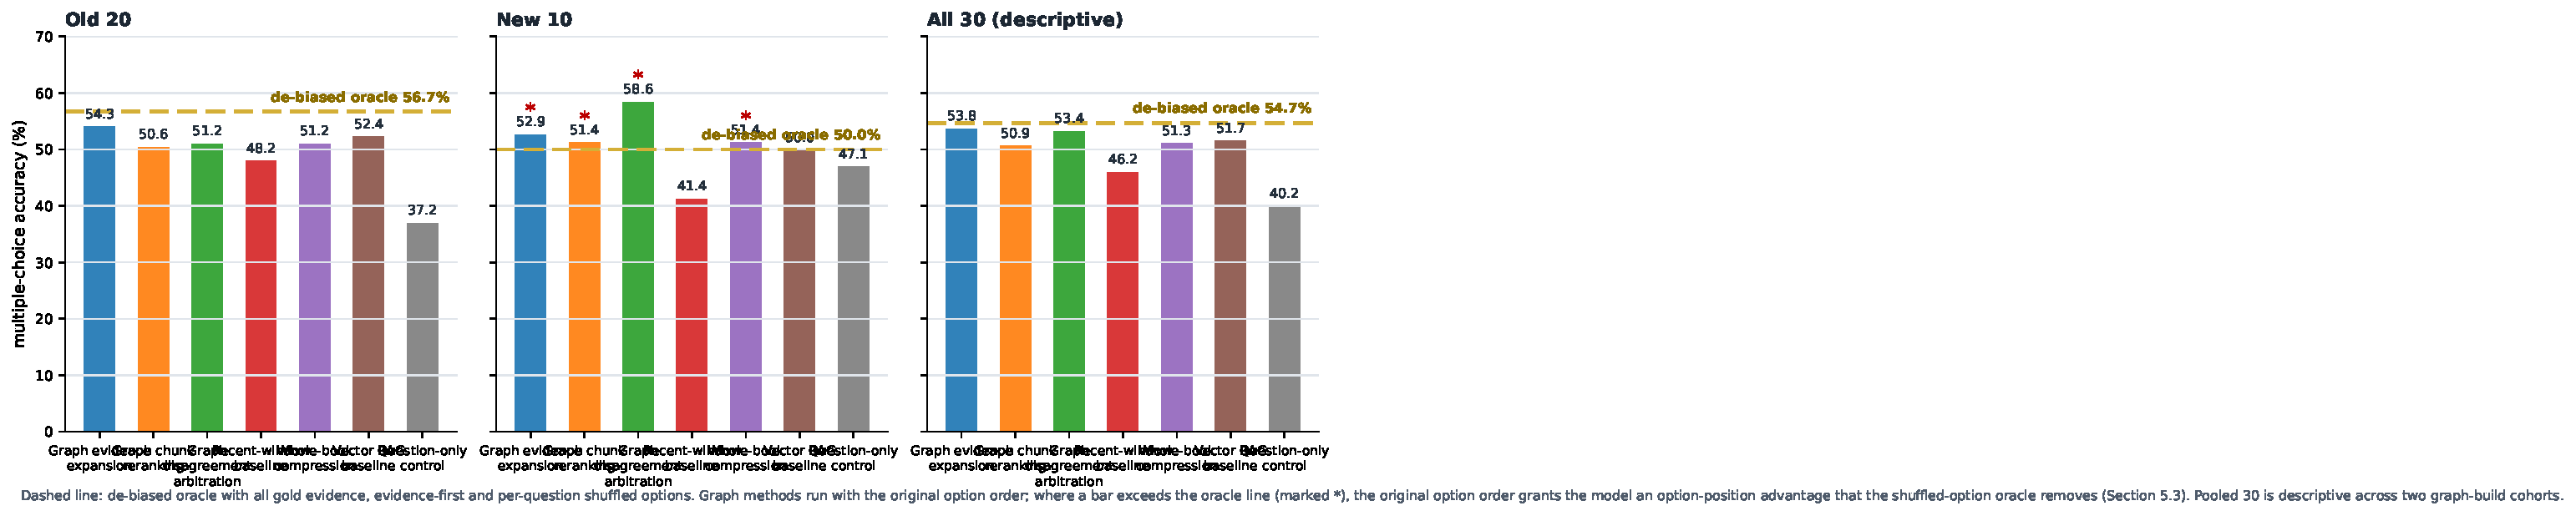
\includegraphics[width=\linewidth]{fig_main_accuracy.pdf}
\caption{
七个非预言机条件的分队列准确率，虚线为去偏预言机参考线。带``*''的柱超过预言机
线；这些运行使用原始选项顺序，而预言机洗牌选项（第~\ref{sec:discussion}~节），
因此位置优势并不为图谱条件所独有——整书压缩基线也越过了该线。合并值横跨两个
图谱构建队列，仅具描述性。
}
\label{fig:main}
\end{figure}

\subsection{闭源大模型参考点}
\label{sec:closedref}

为给本地 9B 结果定位，表~\ref{tab:closed}~报告同一 old20 队列（164 题）上一个
闭源前沿模型（DeepSeek v4-flash，禁用思维链）的结果。给定整本小说文本它达到
80.5\%；限制到线性的 50{,}000 字符尾部窗口则降到 54.9\%；仅给题目为 41.5\%。
两点观察：其一，线性历史阅读把即使前沿模型也封顶在 54.9\%，只有读完整本小说才能
跃至 80.5\%——这正是线性访问的代价。其二，本地 9B 模型仅靠图谱导航就达到
54.3\%（表~\ref{tab:main}），以一小部分上下文预算追平了前沿模型的线性尾部阅读
准确率；前沿模型的剩余优势来自大得多的上下文窗口，16\,K 模型无法企及。这是一个
描述性的跨模型参考，而非受控对比：不同模型的内在上限不同，这正是我们主分析把
每个模型与模型特异的去偏预言机比较的原因。

\begin{table}[t]
\centering
\caption{
old20 队列（164 题）上的外部参考点。``线性尾部''指小说最后 50{,}000 字符。
最后一行重复本地 9B 图谱结果以便直接对比。
}
\label{tab:closed}
\begin{tabular}{lcc}
\toprule
条件 & 正确/总数 & 微平均准确率 \\
\midrule
仅题目 & 68/164 & 41.5\% \\
线性尾部（50\,K 字符） & 90/164 & 54.9\% \\
整本小说 & 132/164 & 80.5\% \\
\midrule
图谱引导的证据扩展（本地 9B） & 89/164 & 54.3\% \\
\bottomrule
\end{tabular}
\end{table}

\subsection{图谱导航逼近金标上限}
\label{sec:goldceiling}

核心比较是金标预言机对仅题目对照与三种图谱协议（表~\ref{tab:paired}、
图~\ref{fig:pairwise}）。公平金标预言机比仅题目对照高出 +14.53\,\pp{}（不一致对
63 胜对 29 负，$p=0.0005$，95\% CI $[6.9, 23.4]$\,\pp）。这是证据效应：同一个
9B 模型，在位置中性的协议下得到全部官方线索，准确率提升 14.5 点。图谱引导的
证据扩展只拿到若干图谱推导的段落，却达到 53.8\%，其对预言机的配对差为
$+0.85$\,\pp{}（$p=0.912$；差值按``第一个条件减第二个条件''报告，因此 $+0.85$
对预言机有利）：图谱阅读器与拿到完整金标证据的阅读器在统计上不可区分。
基于图谱的分歧仲裁同样不可区分（$+1.28$\,\pp，$p=0.832$，同样对预言机有利）。

\begin{table}[t]
\centering
\caption{
同一 234 题上的配对对比（精确双侧 McNemar；W/L = 不一致对上的胜/负；95\% CI 为
按小说聚类的 bootstrap）。上块为金标预言机分析；下块为图谱方法对尾窗口基线、
带 Holm 校正 $p$。
}
\label{tab:paired}
\newcolumntype{L}{>{\raggedright\arraybackslash}X}
\newcolumntype{R}{>{\raggedright\arraybackslash}p{2.1cm}}
\small
\begin{tabularx}{\linewidth}{L rrrrR}
\toprule
配对对比 & $\Delta$ & W/L & 精确 $p$ & Holm $p$ & bootstrap 95\% CI \\
\midrule
公平金标 vs.\ 仅题目(简洁) & +14.53pp & 63/29 & \textbf{0.0005} & -- & [6.9, 23.4] \\
公平金标 vs.\ 图谱引导的证据扩展 & +0.85pp & 42/40 & 0.912 & -- & [-5.9, 8.0] \\
公平金标 vs.\ 图谱分歧仲裁 & +1.28pp & 46/43 & 0.832 & -- & [-6.6, 9.7] \\
选项在前金标 vs.\ 仅题目(伪影) & +1.28pp & 43/40 & 0.826 & -- & [-4.9, 7.8] \\
\midrule
证据扩展 vs.\ 尾窗口(合并) & +7.69pp & 47/29 & 0.050 & 0.454 & [2.0, 13.9] \\
分歧仲裁 vs.\ 尾窗口(new10) & +17.14pp & 15/3 & 0.008 & 0.068 & [5.4, 31.9] \\
\bottomrule
\end{tabularx}
\end{table}

\begin{figure}[t!]
\centering
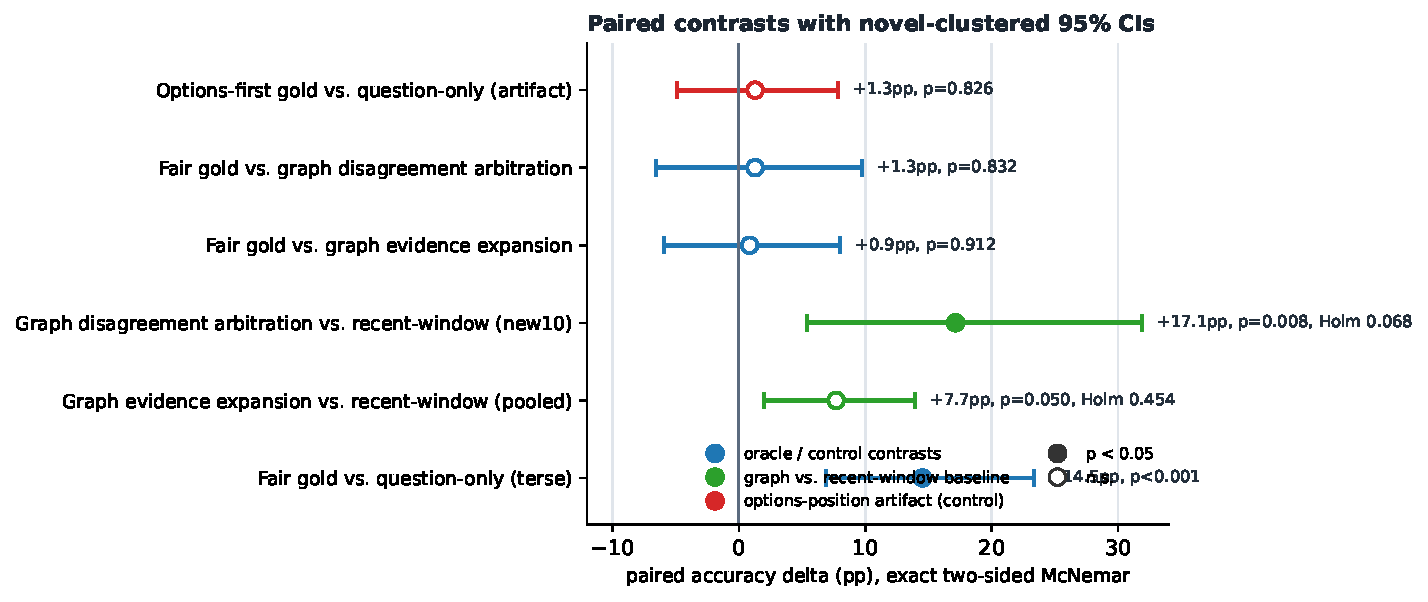
\includegraphics[width=\linewidth]{fig_pairwise.pdf}
\caption{
关键配对对比的森林图。实心标记为 $p<0.05$ 显著；误差条为按小说聚类的
bootstrap 95\% CI。头条证据效应（公平金标 vs.\ 仅题目）为 +14.5\,\pp，而图谱
方法与公平金标预言机不可区分。
}
\label{fig:pairwise}
\end{figure}

\subsection{选项位置锚定是方法学伪影}
\label{sec:danchor}

图~\ref{fig:danchor}~与表~\ref{tab:danchor}（附录）说明了为什么预言机必须去偏。
选项在前金标预言机——全部证据、选项在前、原始顺序——得分为 41.5\%，与仅题目对照
（40.2\%）在统计上不可区分；但这并不是``证据无益''的结果：当金标答案为 D 时预言
机有 79.4\% 的正确率（234 题中金标字母为 D 的有 65 题），而 A--C 只有
21.8--40.0\%，达到或低于对照的逐字母水平。9B 模型锚定于选项的位置。洗牌选项并
把证据提前可以消除该伪影：逐字母准确率趋于平坦（公平预言机 A 55.2\%、B 47.2\%、
C 53.4\%、D 61.5\%），所选字母分布也与内容隐含的金标字母分布一致。

\begin{figure}[t!]
\centering
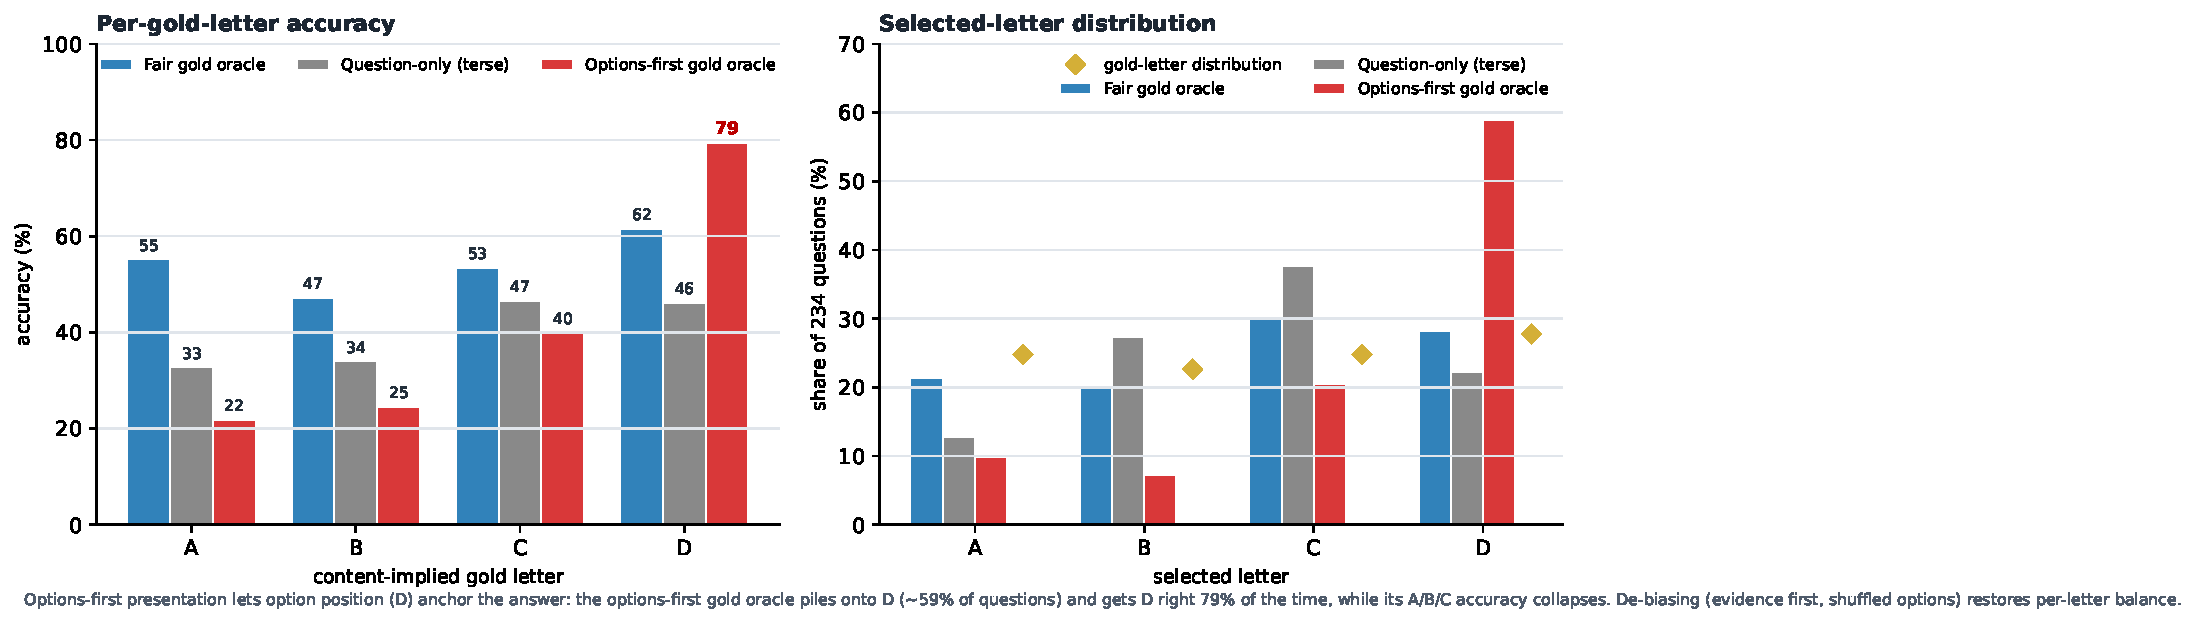
\includegraphics[width=\linewidth]{fig_d_anchoring.pdf}
\caption{
\textbf{左：}逐金标字母准确率。选项在前预言机 A--C 为 21.8--40.0\%（达到或低于
对照的逐字母水平），但 D 为 79.4\%（高亮），即锚定特征。\textbf{右：}所选字母分布
（占题目比例）；选项在前预言机涌向 D（约 59\%），而去偏预言机跟随内容隐含的金标
字母分布。
}
\label{fig:danchor}
\end{figure}

\subsection{队列异质性}
\label{sec:heterogeneity}

两个冻结队列行为差异很大，这决定了合并数字。在 old20 队列中，金标证据压倒性地
位于图的 2-核内——金标重叠率为 53.7\%，其他节点仅 18.2\%（富集 2.95，比值比
5.21），图谱检索只达到 16.3\% 的金标段落。在 new10 队列中图谱构建完整得多：
检索到 73.2\% 的金标段落，富集 1.61（比值比 2.32），最佳图谱协议达到 58.6\%
（其较保守协议下的去偏预言机为 50.0\%）。两个队列因此界定了图谱流水线失效与
成功的两种模式。

\subsection{难题子集表现}
\label{sec:q0hard}

仅题目对照答错的 140 题正是真正需要证据的题。在该子集上，公平金标预言机达到
47.1\%（66/140）；图谱原生分块重排为 45.0\%，图谱引导的证据扩展 42.9\%，基于
图谱的分歧仲裁 41.4\%。每种图谱协议都超过尾窗口基线（33.6\%）以及压缩（37.1\%）
和 RAG（36.4\%）基线。在难题上与预言机的差距来自图谱流水线丢失证据，而非阅读器
推理能力不足。

\subsection{配对统计汇总}
\label{sec:stats}

在九个图谱对基线对比这一族中，图谱引导的证据扩展对尾窗口是最强的合并信号
（+7.69\,\pp，$p=0.050$，Holm 校正 $p=0.454$）；在 new10 队列上，基于图谱的
分歧仲裁对尾窗口为 +17.14\,\pp（15 胜对 3 负，$p=0.008$，Holm 校正
$p=0.068$）。Holm 校正对 9 对比族是保守的；我们全文报告精确值与校正值。

% ============================================================================
\section{讨论}
\label{sec:discussion}

\textbf{图谱导航把位置转化为拓扑。}头条结果背后的机制在图~\ref{fig:schematic} 中
可见：对固定 16\,K 上下文的模型，问题不在于线索是否存在于书中，而在于阅读器能否
到达它。目标在线性位置 0.05 还是 0.95，一步图跳的代价相同。图谱引导的证据扩展
用几百个 token 的图谱选择证据就追平了拿到完整官方线索集的阅读器——图谱实际上
是一张非线性索引，让模型把小的上下文花在答案所在之处。

\textbf{协议不对称对图谱方法有利。}公平金标预言机洗牌选项并先呈现证据；图谱协议
运行原始选项顺序。对位置敏感的 9B 模型来说洗牌更难，因此预言机的 54.7\% 是保守
上限。这就是为什么在 new10 队列上图谱方法可以超过去偏预言机线
（图~\ref{fig:main}）：在原始选项顺序下，同样的证据对这个模型更值钱。这种不对称
意味着我们``与上限不可区分''的主张若非如此，至少是保守的。

\textbf{图谱在哪里丢失。}图谱方法与预言机的差距几乎全部来自检索侧：在难题上图谱
协议达到 41--45\%，预言机为 47.1\%；队列异质性显示差距恰好在图谱召回最低处最大
（old20：16.3\% 金标召回）。基于图谱的分歧仲裁通过运行两个阅读器并仲裁其分歧来
部分找回丢失的证据，这正是它在更强的 new10 队列上成为最佳协议（58.6\%）的原因。

\textbf{小模型是正确的试验场。}拥有大上下文和强指令跟随的前沿模型或许能在窗口内
``线性搜索''；9B 模型配 16\,K 上下文做不到。我们的结果表明图谱原语对正是这一
领域最重要——本地、设备端、成本敏感部署的领域。

\textbf{迈向非线性结构化记忆。}我们的图谱实现了一个一般原语：读者通过导航而非
线性扫描来查询的结构化记忆。对长历史的注意力既昂贵又带位置偏置；稀疏索引以一点
检索代价换取对位置的自由。这一方向会缩放：一个 1M token 上下文的模型要在一个
100M token 的语料或长期记忆上推理，面临的正是 16\,K 模型面对半百万字符小说时的
问题——证据就在历史的某处，但读者负担不起把它全看完。如果导航在这里让小型模型
逼近了它的证据上限，同一个非线性索引或许也能让大得多的模型在比其窗口大两个数量级
的历史上逼近它们各自的上限。

% ============================================================================
\section{局限}
\label{sec:limitations}

\textbf{异质图谱流水线。}两个队列使用不同的冻结图谱构建；合并数字仅具描述性，
分队列结果必须分开阅读。需要单一统一的图谱流水线才能让合并主张更强。

\textbf{语料上的探索性开发。}图谱协议是在这 30 部小说上开发的；固定 9B 模型和
冻结图谱减少了但没有消除选择偏差。金标与基线条件独立于图谱开发，这保护了上限
比较。

\textbf{单一模型。}所有结论只针对一个 9B 检查点。去偏协议与上限比较应当可以迁移，
但具体数值是模型特异的。

\textbf{词汇级金标匹配。}金标证据按数据集的线索位置与段落匹配；金标预言机看到
官方线索集，而不一定是每个可能有帮助的句子。

\textbf{没有注意力级因果。}我们展示的是准确率差异而非机制；我们没有追踪注意力
到图谱选择证据与线性证据。

\textbf{污染细节。}图谱由整本小说构建，因此图谱节点可能触及答案区域；图谱协议
可以浮现官方线索集之外的内容。这使得预言机比较趋于保守（预言机限于官方线索），
但也意味着图谱自身的上限不受官方线索集约束。

% ============================================================================
\section{更广泛影响}
\label{sec:impact}

这是针对公有领域侦探小说的类合成 QA 的低风险研究；无用户数据，不生成有害内容。
最主要的可迁移发现是方法学层面的：\emph{小型模型的多项选择评估对选项顺序敏感}，
不洗牌选项的金标/预言机运行会产生系统性误导的上限（D 上 79.4\%，其余
21.8--40.0\%）。我们建议对长上下文系统的 MCQ 评估用固定种子洗牌选项，并在估计
证据上限时先呈现证据再呈现选项。图谱检索原语本身在上下文预算紧张的场景下的文档
QA 中有直接应用。

% ============================================================================
\section{结论}
\label{sec:conclusion}

我们表明，非线性知识图谱检索系统能让小型、固定上下文的模型在长侦探小说推理上
逼近证据上限。在去偏协议下，金标预言机是真正的上限（比仅题目对照高
+14.5\,\pp），图谱引导的证据扩展与之在统计上不可区分（$p=0.912$），而三种不同
的图谱协议在真正需要证据的题目上都优于线性历史基线。我们还记录了一个使朴素金标
预言机不可靠的选项位置锚定伪影。对上下文预算紧张的小模型而言，图谱导航是线性
搜索的一种廉价而有效的替代。放眼长远，我们把图谱视为非线性结构化记忆的最简
形式：一种稀疏索引，让模型把注意力花在答案所在之处，与位置无关。线性访问的瓶颈
不会随窗口增大而消失，因此我们预期当模型走向百万 token 上下文、处理上亿 token
甚至更多的语料与记忆时，这一原语会更加重要。

% ============================================================================
\bibliographystyle{plainnat}
\bibliography{references}

% ============================================================================
\appendix
\section{完整分队列结果}
\label{app:full}

表~\ref{tab:full-old20}、\ref{tab:full-new10}~与~\ref{tab:full-pooled}~给出全部
12 个条件在三个队列上的正确数/总数与微平均准确率；表~\ref{tab:preserve}~给出各
方法在仅题目对照答对的题目上的保留率（合并）。

\begin{table}[t]
\centering
\caption{完整分队列结果（old20，164 题）}
\label{tab:full-old20}
\small
\begin{tabular}{lcc}
\toprule
方法 & 正确/总数 & 微平均准确率 (old20) \\
\midrule
公平金标预言机（金标上限） & 93/164 & 56.7\% \\
金标预言机（证据在前，原始顺序） & 97/164 & 59.1\% \\
金标预言机（选项在前，洗牌） & 88/164 & 53.7\% \\
选项在前金标预言机 & 63/164 & 38.4\% \\
图谱引导的证据扩展 & 89/164 & 54.3\% \\
图谱原生分块重排 & 83/164 & 50.6\% \\
基于图谱的分歧仲裁 & 84/164 & 51.2\% \\
尾窗口基线 & 79/164 & 48.2\% \\
整书压缩基线 & 84/164 & 51.2\% \\
向量检索(RAG)基线 & 86/164 & 52.4\% \\
仅题目对照(简洁指令) & 68/164 & 41.5\% \\
仅题目对照 & 61/164 & 37.2\% \\
\bottomrule
\end{tabular}
\end{table}

\begin{table}[t]
\centering
\caption{完整分队列结果（new10，70 题）}
\label{tab:full-new10}
\small
\begin{tabular}{lcc}
\toprule
方法 & 正确/总数 & 微平均准确率 (new10) \\
\midrule
公平金标预言机（金标上限） & 35/70 & 50.0\% \\
金标预言机（证据在前，原始顺序） & 38/70 & 54.3\% \\
金标预言机（选项在前，洗牌） & 35/70 & 50.0\% \\
选项在前金标预言机 & 34/70 & 48.6\% \\
图谱引导的证据扩展 & 37/70 & 52.9\% \\
图谱原生分块重排 & 36/70 & 51.4\% \\
基于图谱的分歧仲裁 & 41/70 & 58.6\% \\
尾窗口基线 & 29/70 & 41.4\% \\
整书压缩基线 & 36/70 & 51.4\% \\
向量检索(RAG)基线 & 35/70 & 50.0\% \\
仅题目对照(简洁指令) & 26/70 & 37.1\% \\
仅题目对照 & 33/70 & 47.1\% \\
\bottomrule
\end{tabular}
\end{table}

\begin{table}[t]
\centering
\caption{完整分队列结果（合并，234 题）}
\label{tab:full-pooled}
\small
\begin{tabular}{lcc}
\toprule
方法 & 正确/总数 & 微平均准确率 (合并) \\
\midrule
公平金标预言机（金标上限） & 128/234 & 54.7\% \\
金标预言机（证据在前，原始顺序） & 135/234 & 57.7\% \\
金标预言机（选项在前，洗牌） & 123/234 & 52.6\% \\
选项在前金标预言机 & 97/234 & 41.5\% \\
图谱引导的证据扩展 & 126/234 & 53.8\% \\
图谱原生分块重排 & 119/234 & 50.9\% \\
基于图谱的分歧仲裁 & 125/234 & 53.4\% \\
尾窗口基线 & 108/234 & 46.2\% \\
整书压缩基线 & 120/234 & 51.3\% \\
向量检索(RAG)基线 & 121/234 & 51.7\% \\
仅题目对照(简洁指令) & 94/234 & 40.2\% \\
仅题目对照 & 94/234 & 40.2\% \\
\bottomrule
\end{tabular}
\end{table}

\begin{table}[t]
\centering
\caption{在仅题目对照答对题目上的保留率（合并）}
\label{tab:preserve}
\begin{tabular}{lc}
\toprule
方法 & 对照答对题的保留率 \\
\midrule
图谱引导的证据扩展 & 70.2\% \\
图谱原生分块重排 & 59.6\% \\
基于图谱的分歧仲裁 & 71.3\% \\
尾窗口基线 & 64.9\% \\
整书压缩基线 & 72.3\% \\
向量检索(RAG)基线 & 74.5\% \\
选项在前金标预言机 & 57.4\% \\
\bottomrule
\end{tabular}
\end{table}

\section{去偏金标分析（逐字母与分布）}
\label{sec:danchor-app}
\begin{table}[t]
\centering
\caption{
去偏与对照运行的逐金标字母准确率（左）与所选字母分布（右），并附内容隐含的金标
字母分布供参考。选项在前预言机的 D 尖峰是锚定伪影。
}
\label{tab:danchor}
\small
\begin{tabular}{lcccc}
\toprule
运行 & A & B & C & D \\
\midrule
公平金标预言机 & 55.2\% & 47.2\% & 53.4\% & 61.5\% \\
仅题目对照(简洁指令) & 32.8\% & 34.0\% & 46.6\% & 46.2\% \\
选项在前金标预言机 & 21.8\% & 24.5\% & 40.0\% & \textbf{79.4}\% \\
\bottomrule
\end{tabular}

\vspace{6pt}
\begin{tabular}{lcccc}
\toprule
运行 & A & B & C & D \\
\midrule
公平金标预言机 & 50 (21.4\%) & 47 (20.1\%) & 71 (30.3\%) & 66 (28.2\%) \\
仅题目对照(简洁指令) & 30 (12.8\%) & 64 (27.4\%) & 88 (37.6\%) & 52 (22.2\%) \\
选项在前金标预言机 & 23 (9.8\%) & 17 (7.3\%) & 48 (20.5\%) & 138 (59.0\%) \\
金标字母分布 & 58 (24.8\%) & 53 (22.6\%) & 58 (24.8\%) & 65 (27.8\%) \\
\bottomrule
\end{tabular}

\vspace{2pt}\begin{scriptsize}
括号内为占 234 题的比例。选项在前金标预言机无论内容如何都涌向 D（138/234 =
59\% 的题目），而去偏的公平金标预言机与内容隐含的金标分布一致。选项在前预言机在
8 题上拒绝选择字母（该行和为 226）。
\end{scriptsize}
\end{table}

\section{图结构分析}
\label{app:graph}
\begin{figure}[t!]
\centering
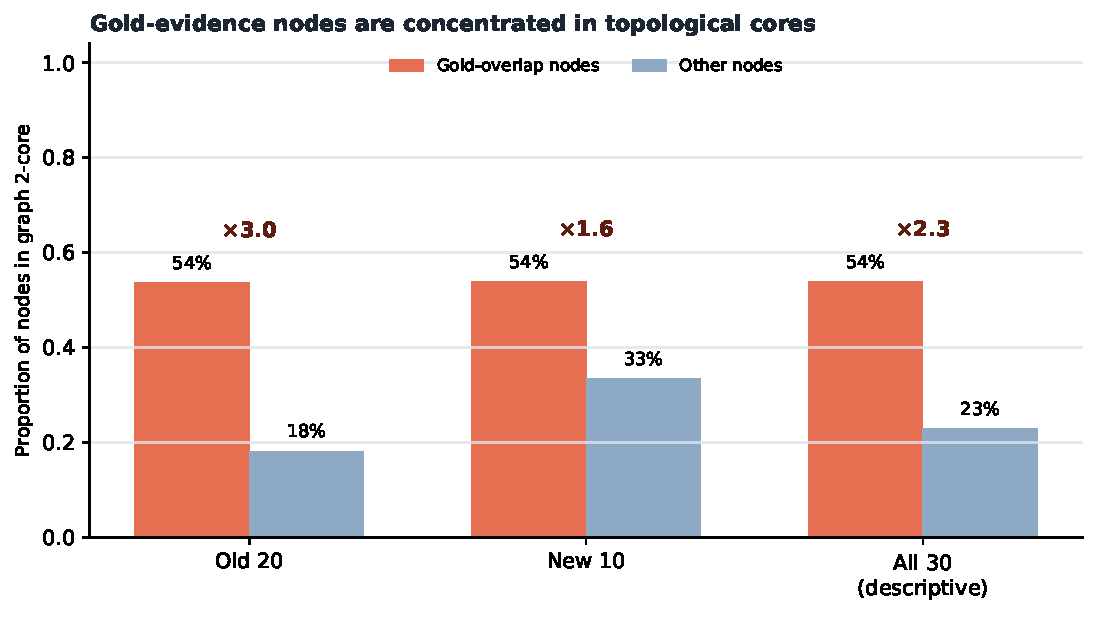
\includegraphics[width=0.82\linewidth]{fig_core_enrichment.pdf}
\caption{
金标重叠节点集中于图的拓扑 2-核。比率为各队列全部图节点上的微平均；``$\times$''
标签为金标/其他节点的比率（富集）。
}
\label{fig:coreenrichment}
\end{figure}

\begin{figure}[t!]
\centering
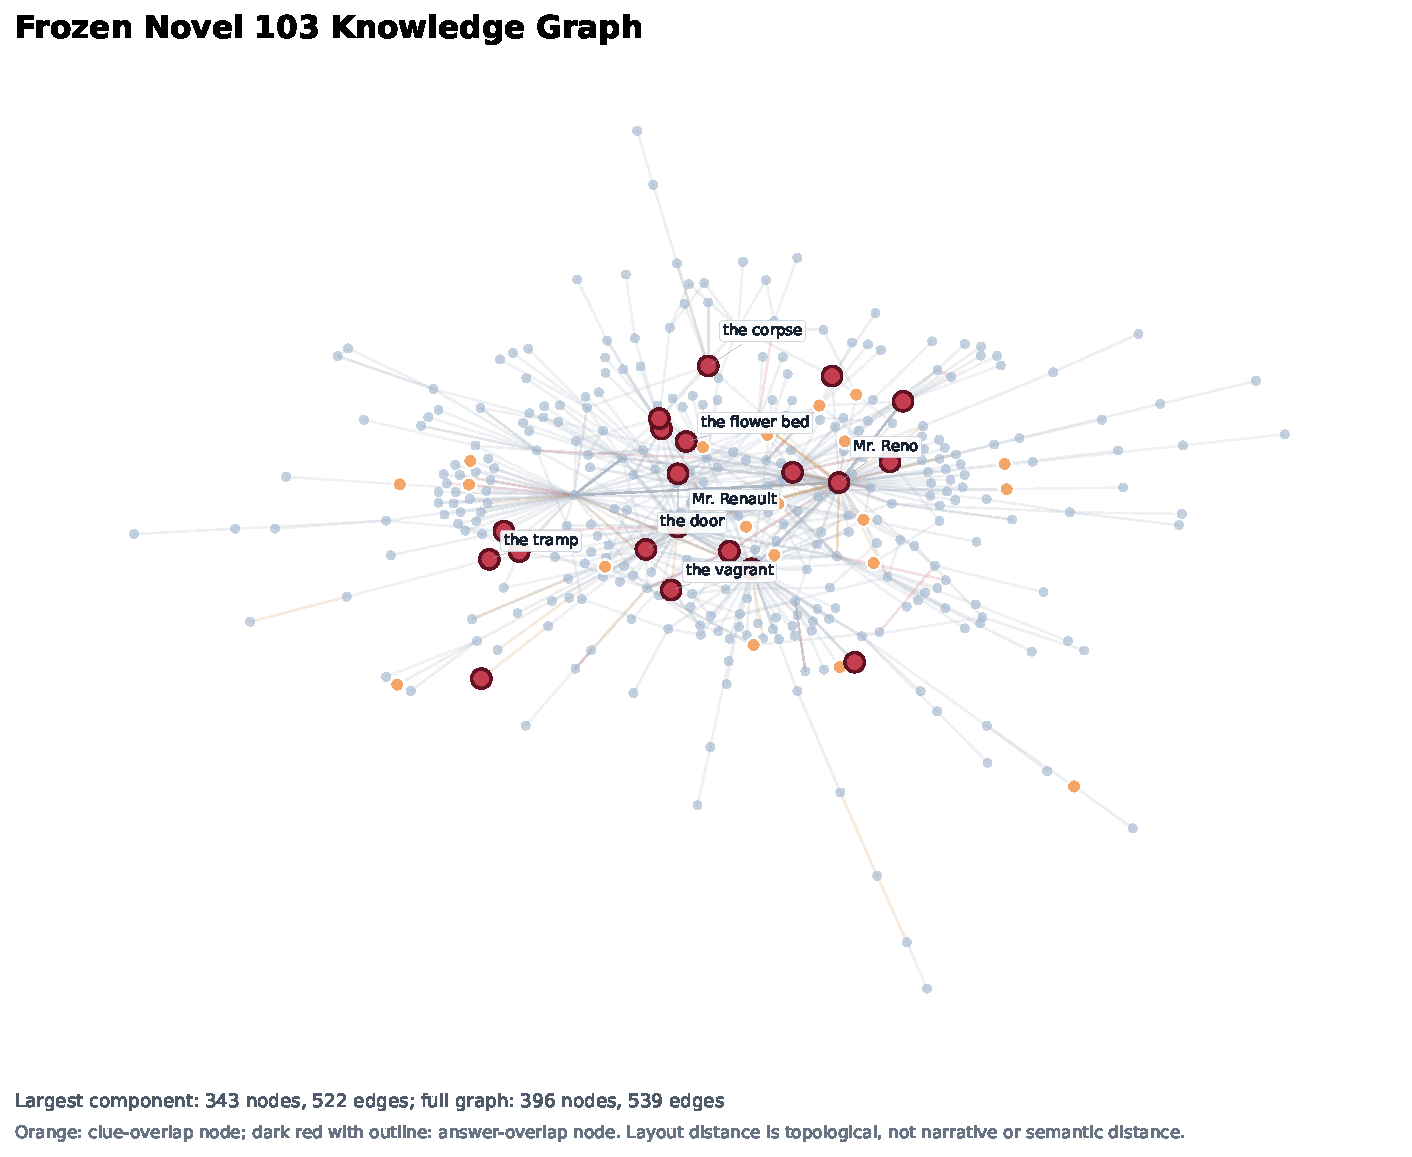
\includegraphics[width=0.55\linewidth]{fig_force_novel103.pdf}
\caption{
一部小说的冻结力导向图（节点数 n、边数 m 如标注）。橙色节点与金标证据重叠；
红色节点与答案重叠。虚线圆标出拓扑核。力导向距离是拓扑的，不是叙事或语义的。
}
\label{fig:force}
\end{figure}

\end{document}
